% Section content template for individual Educative lessons
% This file contains the actual content for a specific section
% Generated from Educative API section content

% Section: Class Diagram for the Airline Management System
% Section ID: 5381527174381568
% Section Slug: class-diagram-for-the-airline-management-system
% Generated: 2025-12-14T13:17:47.041852

In the class diagram, we will first design and create the system's classes, abstract classes, and interfaces. Then , we'll identify the relationship between classes by all the requirements of the airline management system.

\subsection{Components of an airline management system}\label{m6SXYWgpl0gNOj5jctoDv}
\\
In this section, we'll define the classes for an airline management system. As mentioned earlier, we will design the system using a bottom-up approach. First , we will create the classes of small components. Next
, we will integrate these components and create the class diagram for the entire system.

\subsubsection{Account}\label{cC4t1-Ahq0pkxgbZcnSNN}
\\
The \texttt{Account} class identifies the username and ID of an airline management system user. The class definition is represented below:

\begin{figure}[htbp]
 \centering
 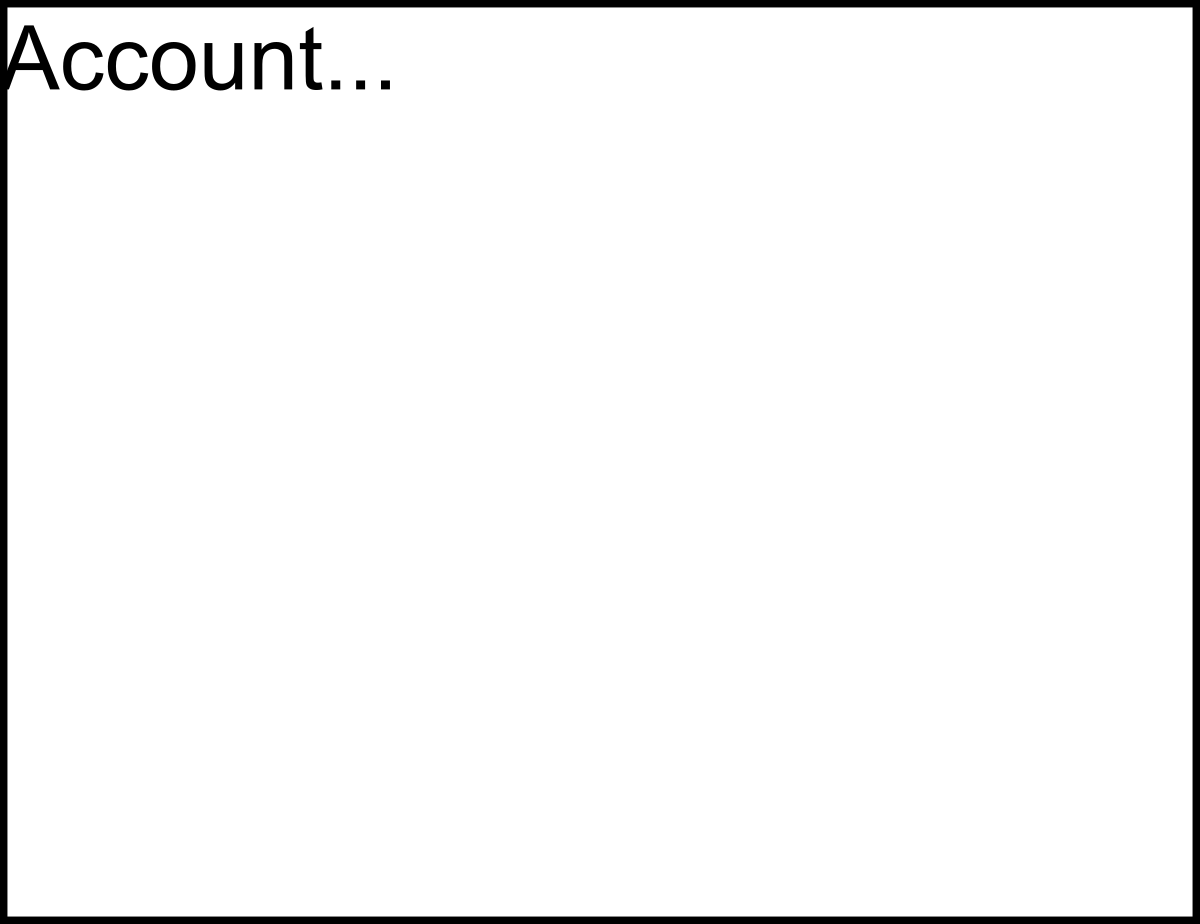
\includegraphics[width=0.5\textwidth]{Images/chapter_25/section_5381527174381568/5626337760116736.png}
 \caption{The Account class}
\end{figure}

\subsubsection{Person}\label{XVzn0KgzobKkiraehnHGg}
\\
A \texttt{Person} is an abstract class used to store information related to a person, such as a name, email, phone number, etc. In this class, the \texttt{Address} object type specifies the person's address. There can be four types of accounts in the system:

\begin{itemize}
\item
\texttt{Admin}\textbf{:} This class manages the overall system, including flight and aircraft records.
\item
\texttt{Crew}\textbf{:} This class views assigned flights in the system.
\item
\texttt{FrontDeskOfficer}\textbf{:} This class manages passenger reservations.
\item
\texttt{Customer}\textbf{:} This class displays flight schedules and allows users to reserve or cancel flight reservations.
\end{itemize}
\\
The relationship diagram for these classes is shown below:

\begin{figure}[htbp]
 \centering
 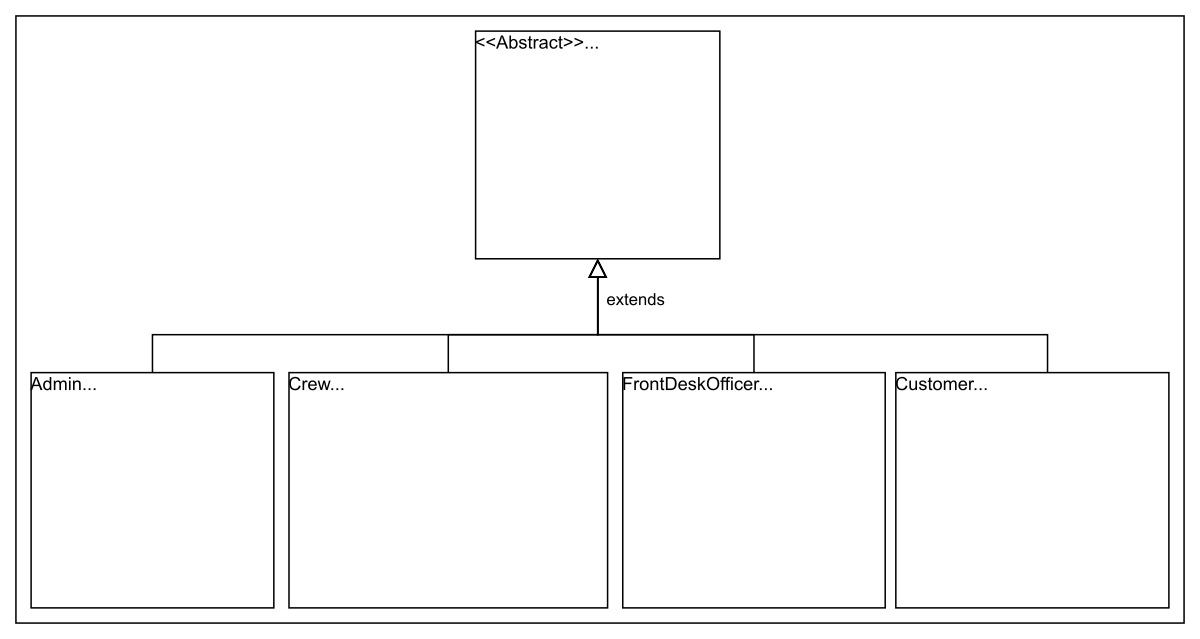
\includegraphics[width=0.5\textwidth]{Images/chapter_25/section_5381527174381568/4903834378698752.png}
 \caption{Person and its derived classes}
\end{figure}

\textbf{R4:} The system should allow customers to check flight details, such as available seats, flight schedules, and departure/arrival times.
\\
\textbf{R5:} The system admin should be able to add new flights and aircraft. The admin should be able to cancel previous flights.
\\
\textbf{R11:} The front desk officer should be able to reserve tickets, create itineraries, and make flight payments for the customer.
\\
\textbf{R12:} The flight crew should be able to view the schedule for their assigned flights.

\subsubsection{Airline, airport, and aircraft}\label{Pj_YekJgAG3MPUjXwXnrp}
\\
The \texttt{Airline} class has attributes such as a name and an airline code to distinguish it from other airlines. It is a crucial component of the airline management system.
\\
Each airline operates out of different airports. Therefore, we need the \texttt{Airport} class to keep track of all the airports in the system.
\\
Airlines own or hire aircraft to carry out their flights. The
\texttt{Aircraft} class has attributes such as name, model, and manufacturing year, among others.
\\
Here's a visual representation of these classes:

\begin{figure}[htbp]
 \centering
 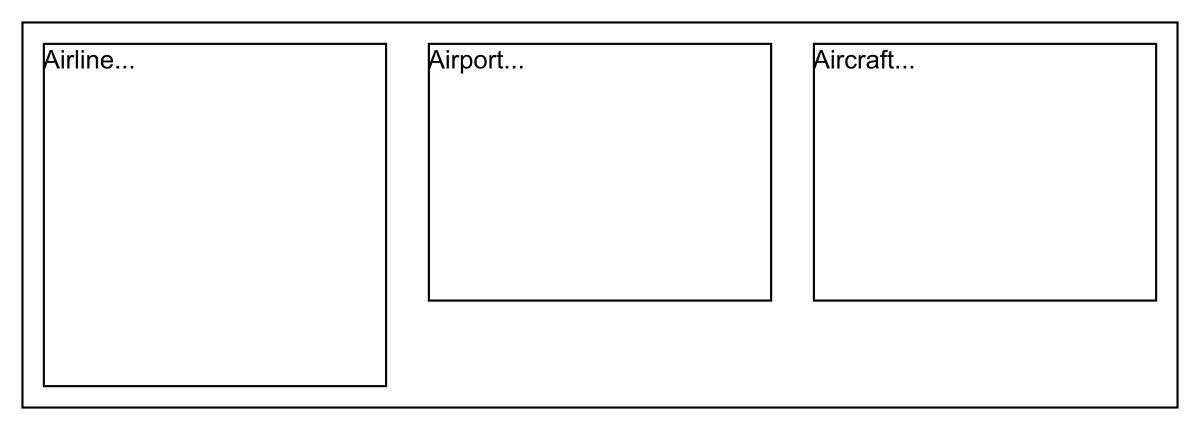
\includegraphics[width=0.5\textwidth]{Images/chapter_25/section_5381527174381568/5744006183911424.png}
 \caption{The Airline, Airport, and Aircraft classes}
\end{figure}

\textbf{R6:} An airline should be able to own multiple aircraft, and the admin should be able to add these aircraft to the system.
\\
\textbf{R7:} An airline should be able to operate its flights from different airports.

\subsubsection{Seat and flight seat}\label{A_hOhm_Csr_W4fI8LjmCh}
\\
The \texttt{Seat} class represents a physical seat in the aircraft.~It contains basic information, such as seat number, seat type, and class. The
\texttt{FlightSeat} class is derived from the \texttt{Seat} class and represents the seat assigned to a specific flight instance. It contains the fare for that particular seat and its reference number.
\\
The relationship diagram for these classes is shown below:

\begin{figure}[htbp]
 \centering
 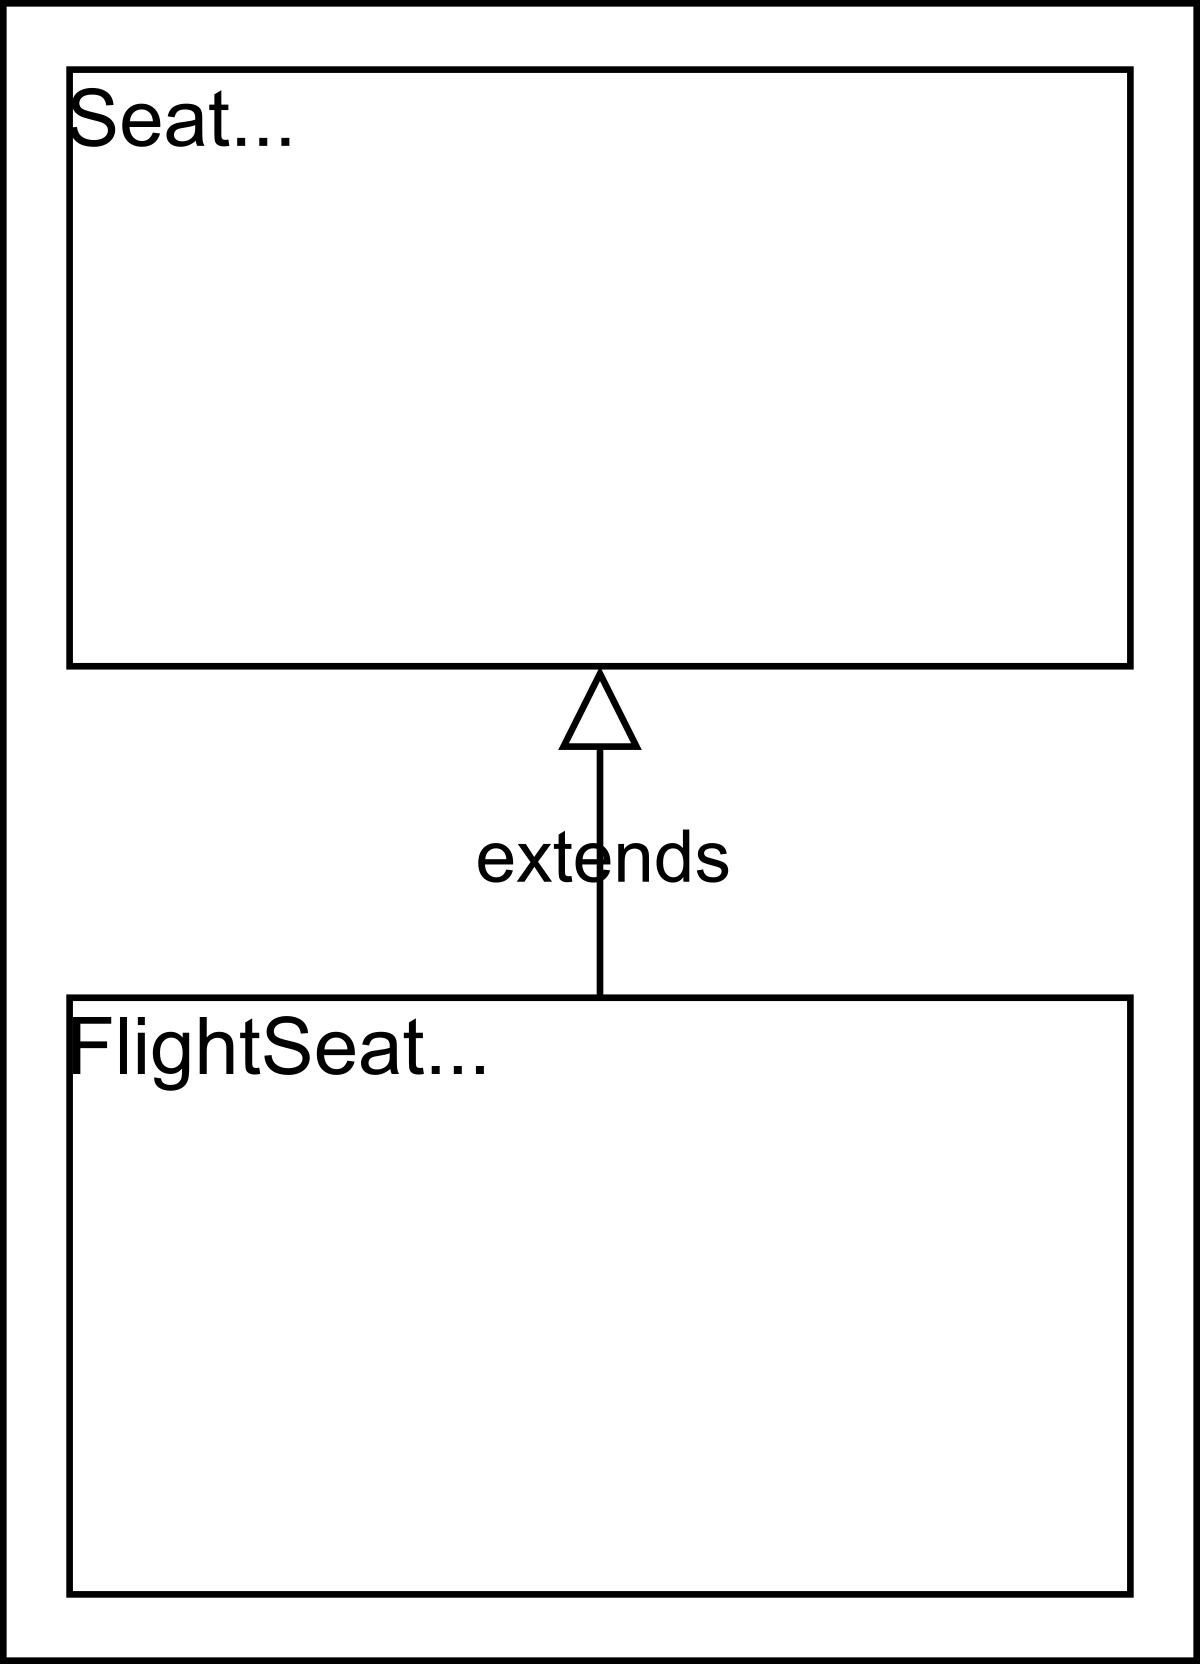
\includegraphics[width=0.5\textwidth]{Images/chapter_25/section_5381527174381568/5673636318150656.png}
 \caption{Seat and its derived class}
\end{figure}

\subsubsection{Flight and flight instance}\label{7gaSwp32yoHRS7lPfGcVQ}
\\
The \texttt{Flight} class contains information about a particular flight, including the flight number, departure and arrival airports, and the duration of the flight. The
\texttt{FlightInstance} class represents a single occurrence of a flight, since a flight can fly multiple days in a week.
\\
These classes are represented below:

\begin{figure}[htbp]
 \centering
 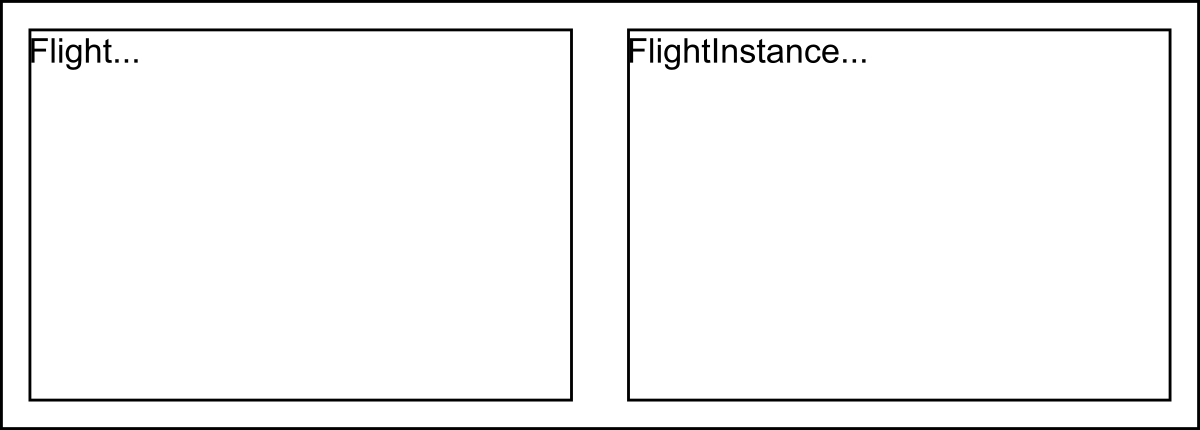
\includegraphics[width=0.5\textwidth]{Images/chapter_25/section_5381527174381568/5385003409342464.png}
 \caption{The Flight and FlightInstance classes}
\end{figure}

\textbf{R1:} A customer should be able to search for flights by date, departure, and destination airport.
\\
\textbf{R4:} The system should allow customers to check flight details, such as available seats, flight schedule, and departure/arrival times.

\subsubsection{Flight reservation}\label{Xqxerk0SdEcxiXlkLk8nX}
\\
The \texttt{FlightReservation} class manages reservations made by customers against a specific flight instance. It has attributes like a unique reservation number, passengers and their assigned seats, and the reservation status.
\\
The UML diagram for this class is given below:

\begin{figure}[htbp]
 \centering
 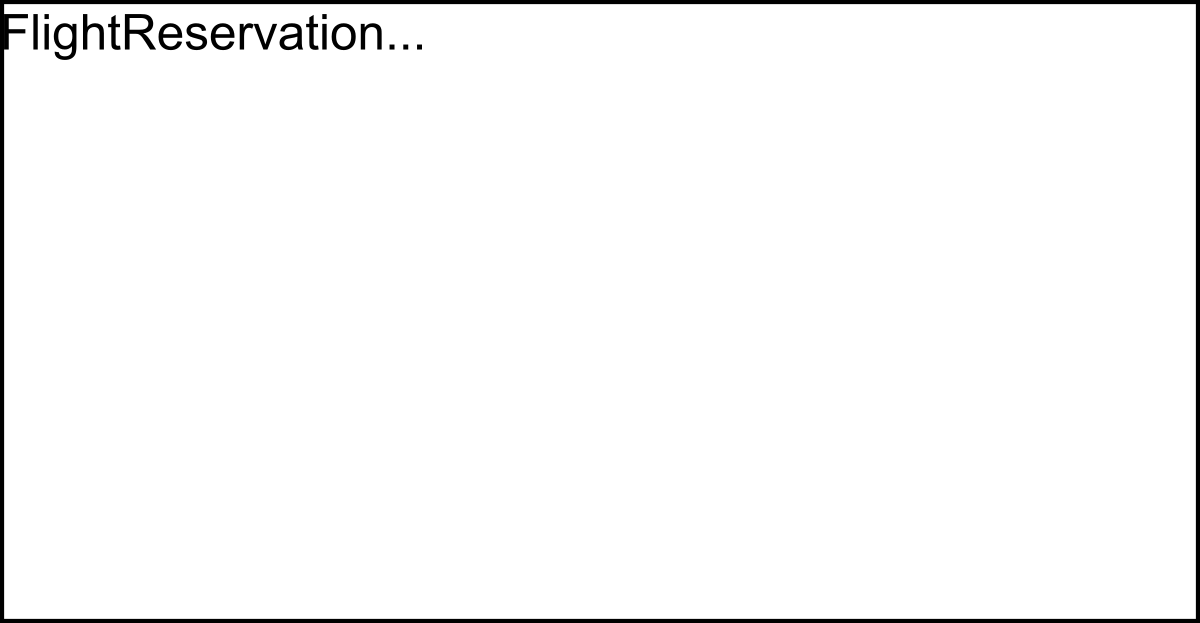
\includegraphics[width=0.5\textwidth]{Images/chapter_25/section_5381527174381568/6382929132650496.png}
 \caption{The FlightReservation class}
\end{figure}

\textbf{R2:} Customers should be able to reserve tickets for available flights and book multiple flights at once.

\subsubsection{Itinerary and passenger}\label{L6I504392SXA5rUdQcC19}
\\
Customers create an itinerary for their travel that contains flight reservations. The
\texttt{Itinerary} class keeps track of all the reservations made, the list of passengers, and the departure/arrival airport.
\\
The \texttt{Passenger} class maintains a record of all individuals with reservations. It also includes the basic travel information of the passenger.
\\
Here's the class diagram for these classes:

\begin{figure}[htbp]
 \centering
 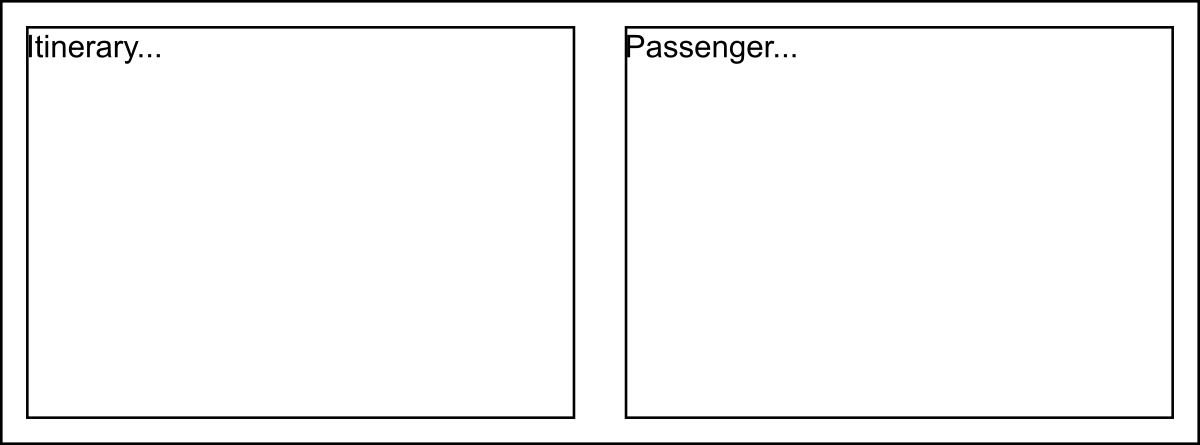
\includegraphics[width=0.5\textwidth]{Images/chapter_25/section_5381527174381568/4623461038424064.png}
 \caption{The Itinerary and Passenger classes}
\end{figure}

\textbf{R2:} Customers should be able to reserve tickets for available flights and book multiple flights at once.

\subsubsection{Search and catalog}\label{rIyUszAGv0myo-sMSw9BM}
\\
The~\texttt{Search}~interface allows customers to search for any flight using the following criteria:

\begin{itemize}
\item
\protect\phantomsection\label{REKZDjbra0SsmtXvQvN4n}
Departure and arrival date and time
\item
\protect\phantomsection\label{saFXz-yJJrKBxAkK3Cn67}
Source and destination airports
\end{itemize}
\\
The \texttt{SearchCatalog} implements the search functionality and contains a list of all flights of the airline. The two classes are shown below:

\begin{figure}[htbp]
 \centering
 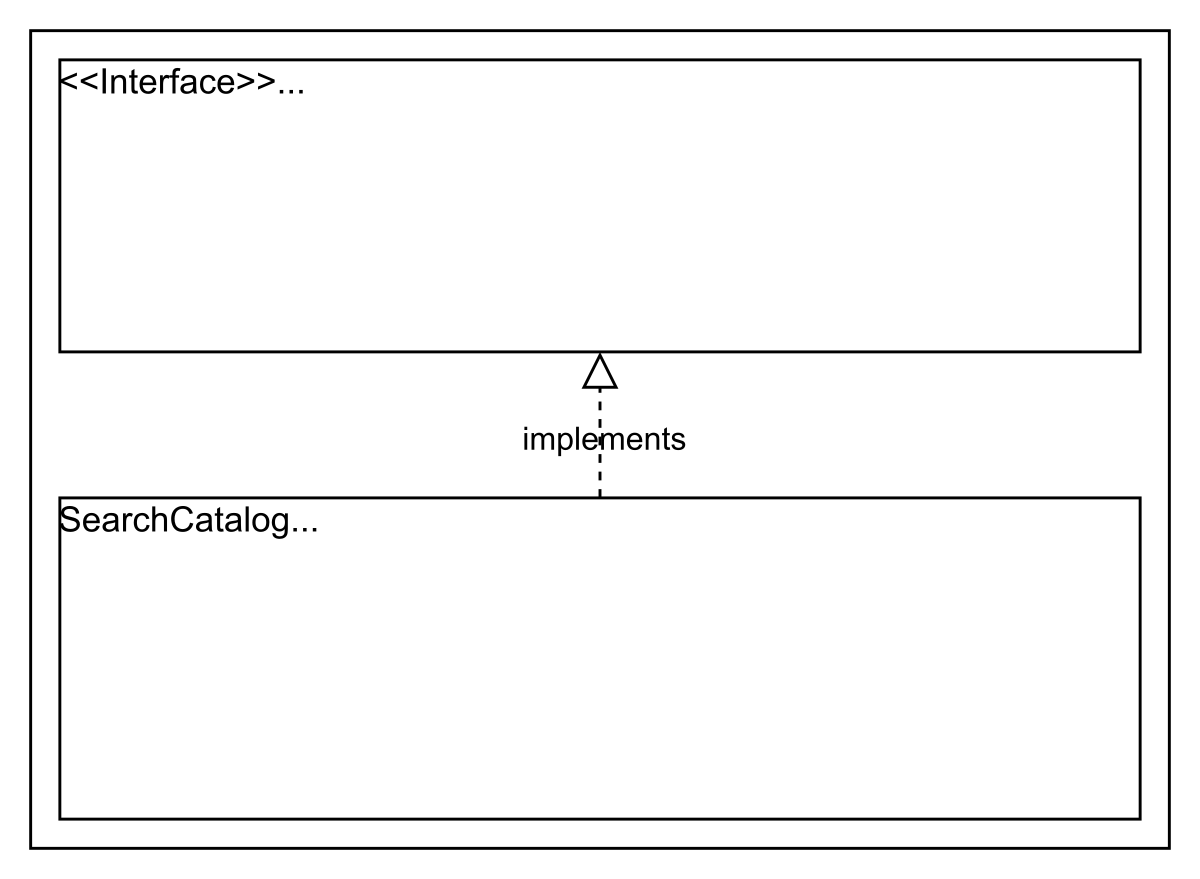
\includegraphics[width=0.5\textwidth]{Images/chapter_25/section_5381527174381568/5228070049808384.png}
 \caption{The Search interface and the SearchCatalog class}
\end{figure}

\textbf{R1:} Customers should be able to search for flights by date, departure, and destination airport.

\subsubsection{Payment}\label{XzReB6haFOdc_kM5xqrQA}
\\
The \texttt{Payment} class will be an abstract class and will have two child classes: \texttt{CreditCard}, and \texttt{Cash}.
\\
The visual representation of these classes is as follows:

\begin{figure}[htbp]
 \centering
 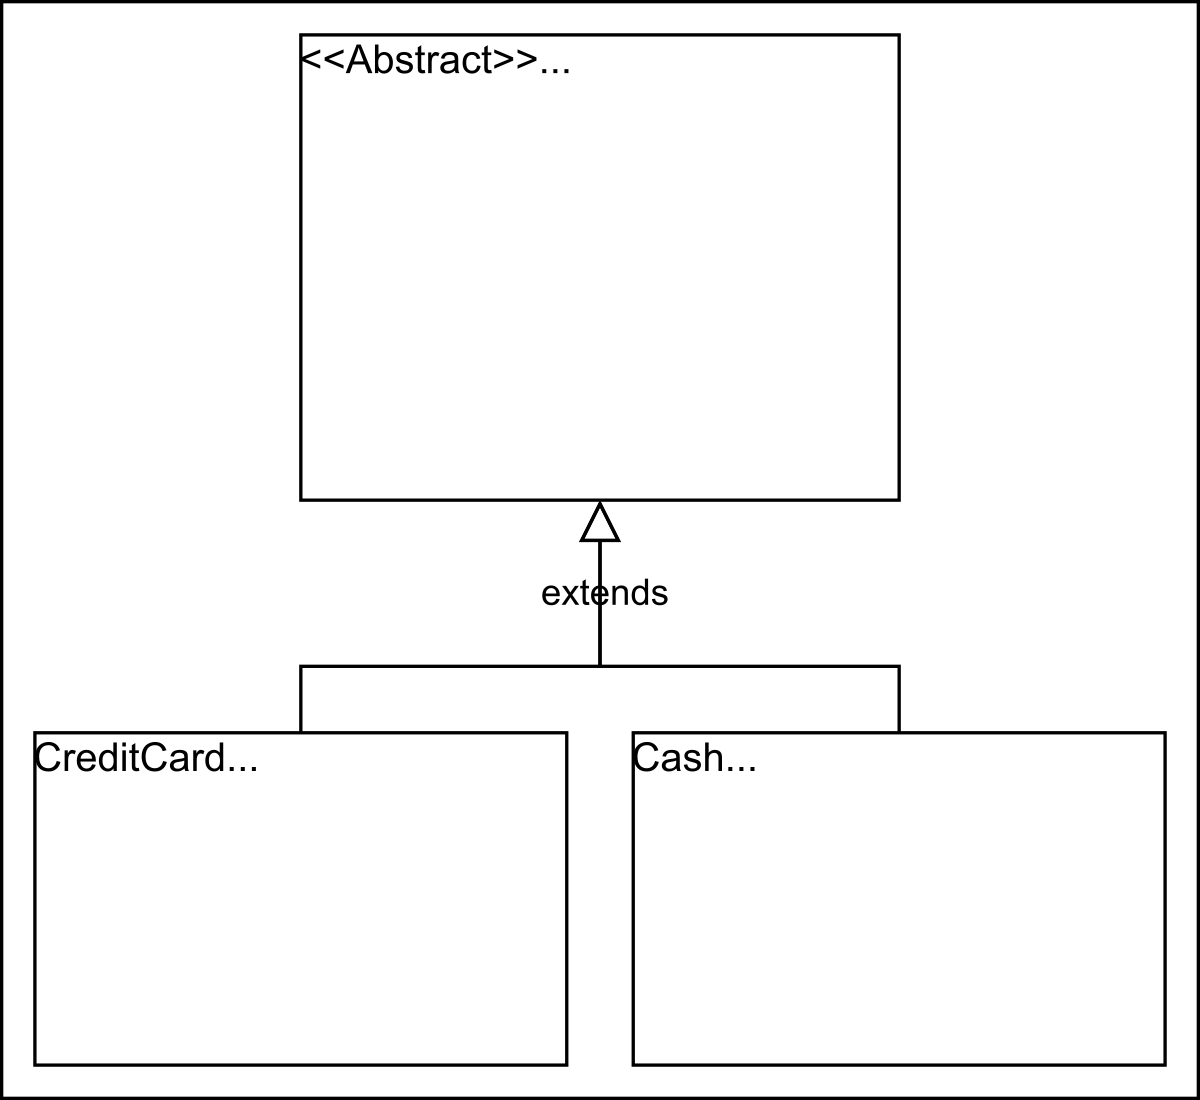
\includegraphics[width=0.5\textwidth]{Images/chapter_25/section_5381527174381568/5648591206219776.png}
 \caption{The Payment and its derived classes}
\end{figure}

\textbf{R9:} The customer should be able to make payments against their flight reservations.

\subsubsection{Notification}\label{7FuE-vRiQ2Hux6ybLOosN}
\\
\texttt{Notification}~is an abstract class, since it can send a notification via email or SMS. It is primarily responsible for sending notifications as needed.
\\
The UML representation of the class is shown below:

\begin{figure}[htbp]
 \centering
 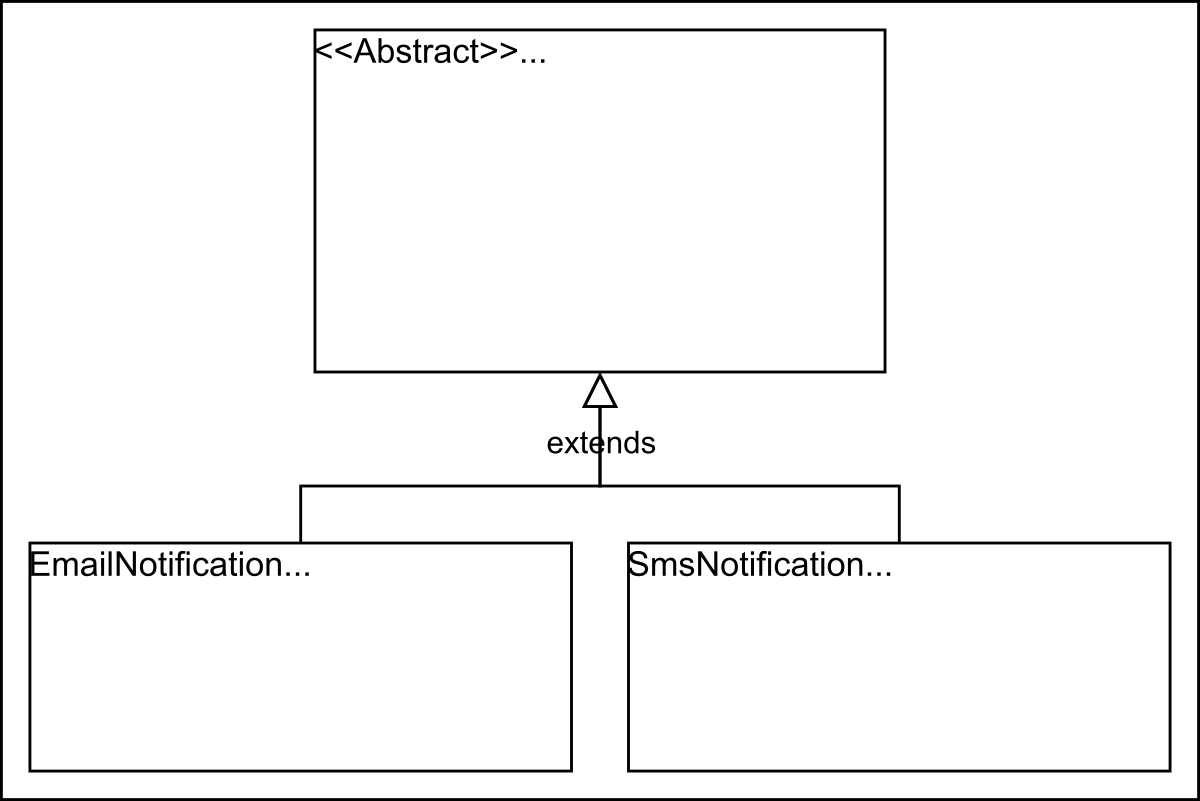
\includegraphics[width=0.5\textwidth]{Images/chapter_25/section_5381527174381568/5217956444504064.png}
 \caption{Notification and its derived classes}
\end{figure}

\textbf{R13:} The system should notify the customer whenever a reservation is made or canceled, or when there is an update regarding their flight.

\subsubsection{Enumerations}\label{ii8ggxura0jzCr2Gmnj6Y}
\\
The enumerations required in the airline management system design are listed below:

\begin{itemize}
\item
\texttt{AccountStatus}\textbf{:} The account status indicates the current status of a customer's account---whether it is active, deactivated, closed, or blocked.
\item
\texttt{SeatStatus}\textbf{:} The seat status tells us whether the seat is available, booked, or a chance seat.
\item
\texttt{SeatType}\textbf{:} The seat type indicates whether the seat is of a regular, accessible, emergency exit, or extra-legroom type.
\item
\texttt{SeatClass}\textbf{:} The seat class indicates whether the seat is in Economy, Economy Plus, Business, or First Class.
\item
\texttt{FlightStatus}\textbf{:} The flight status tracks the flight instance, indicating whether it is active, scheduled, delayed, departed, landed, canceled, diverted, or unknown.
\item
\texttt{ReservationStatus}\textbf{:} The reservation status indicates the current status of the reservation---whether it is requested, pending, confirmed, checked in, or canceled.
\end{itemize}
\\
PaymentStatus\textbf{:} The payment status indicates the current status of the payment---whether it is pending, completed, canceled, failed, declined, or refunded.

\begin{figure}[htbp]
 \centering
 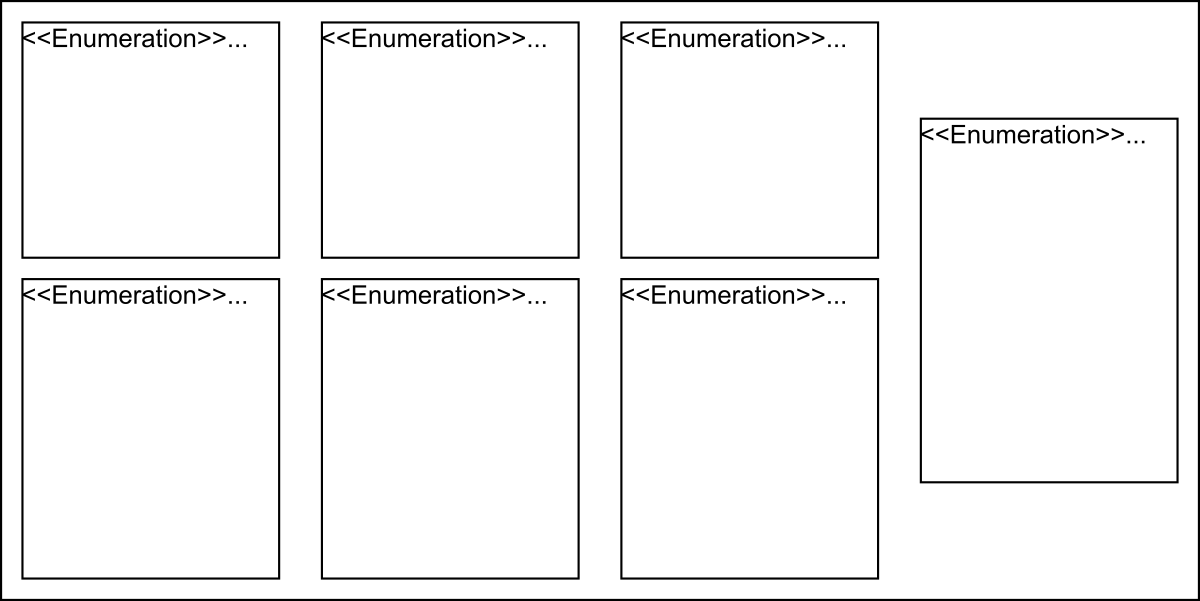
\includegraphics[width=0.5\textwidth]{Images/chapter_25/section_5381527174381568/6013888509509632.png}
 \caption{Enums in the airline management system}
\end{figure}

\subsubsection{Custom data type}\label{MnDHVZdtEzMjuvjmC3fmi}
\\
We need to create a custom data type,~\texttt{Address}, that will store the physical location of any place.

\begin{figure}[htbp]
 \centering
 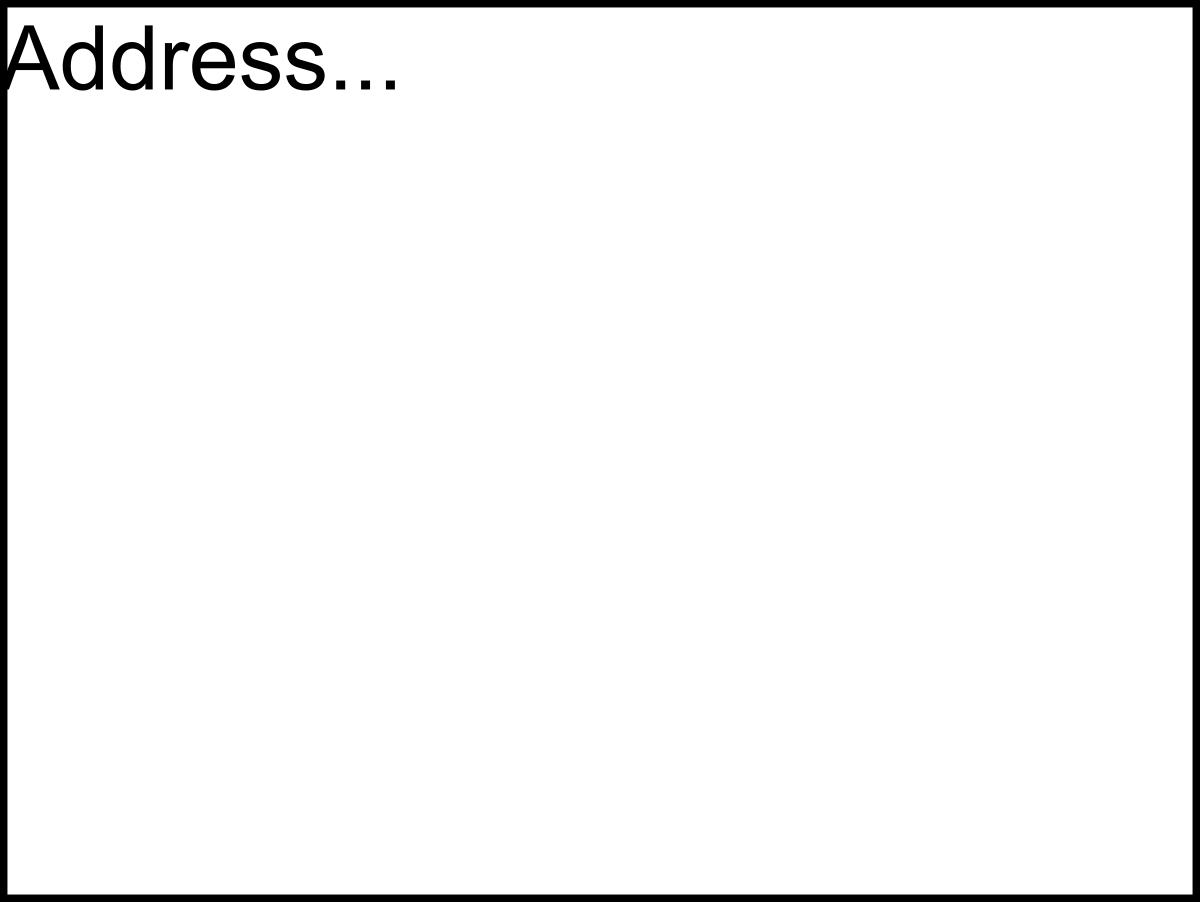
\includegraphics[width=0.5\textwidth]{Images/chapter_25/section_5381527174381568/6119539457916928.png}
 \caption{The Address custom data type}
\end{figure}

\subsection{Relationship between classes}\label{tyhQ4mzKAH5p6Wm5SwLs0}
\\
Now, we'll discuss the relationships between the classes we have defined in our airline management system above.

\subsubsection{Association}\label{fFvB4PDNxRHiQ40A_5Drq}
\\
The class diagram has the following association relationships:
\\
\paragraph{One-way association}\label{hEd0Kf4m3HPXM7yWMTr1I}

\begin{itemize}
\item
\protect\phantomsection\label{gckg7hpAf7veUld_vM6q1}
Both \texttt{FrontDeskOfficer} and \texttt{Customer} classes have a one-way association with the \texttt{Itinerary} class.
\item
\protect\phantomsection\label{5B6geNDP791ZXH9L1MqjA}
The \texttt{FlightReservation} class has a one-way association with the \texttt{FlightInstance}, \texttt{Payment}, and \texttt{Notification} classes.
\item
\protect\phantomsection\label{uML3_Lr8_DNLmPJ67nFF2}
The \texttt{FlightSeat} class has a one-way association with the \texttt{FlightReservation} class.
\item
\protect\phantomsection\label{0iqvStT8l7Ejy634Mzn1Y}
The \texttt{Person} class has a one-way association with the \texttt{Search} interface.
\end{itemize}
\\
\paragraph{Two-way association}\label{VXdnbW2DNHqLyGNR7FwCK}

\begin{itemize}
\item
\protect\phantomsection\label{6JZji_NsYByUtLtZnjE6s}
The \texttt{Airport} class has a two-way association with the \texttt{Flight} class.
\item
\protect\phantomsection\label{lIpFWiQgnGh6Mwd2kxEsy}
Both the \texttt{Aircraft} and \texttt{Crew} classes have a two-way association with the \texttt{FlightInstance} class.
\item
\protect\phantomsection\label{ivsiIEW7Ch6B4JhkVn5qV}
The \texttt{Airline} class has a two-way association with the \texttt{Crew} class.
\end{itemize}

\begin{figure}[htbp]
 \centering
 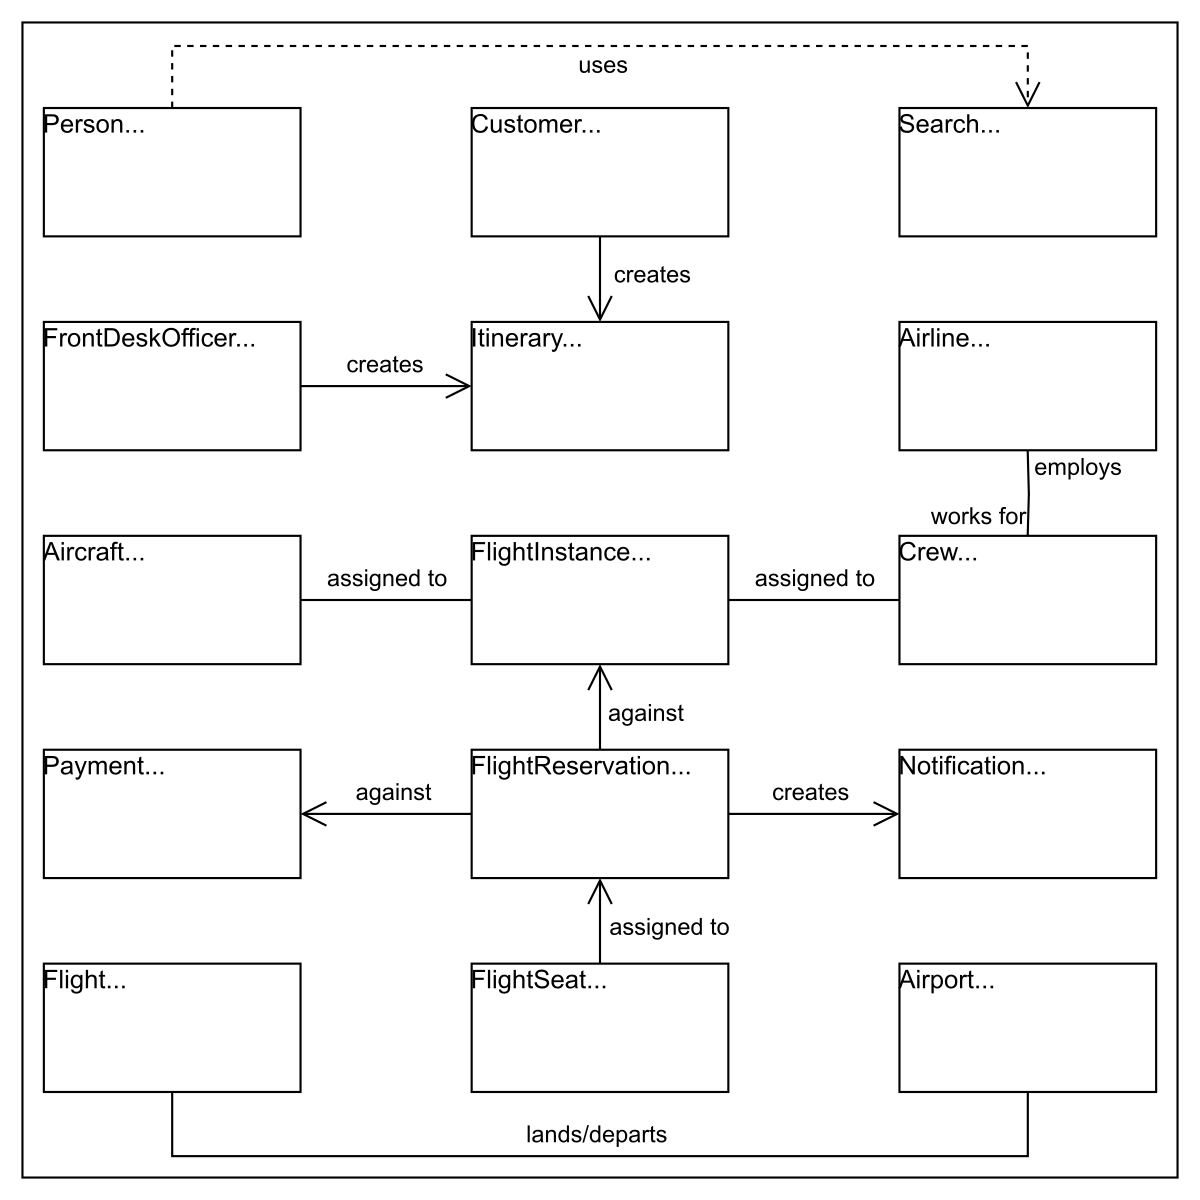
\includegraphics[width=0.5\textwidth]{Images/chapter_25/section_5381527174381568/5836943538388992.png}
 \caption{Association relationship between classes}
\end{figure}

\subsubsection{Aggregation}\label{YY7KnLdnh84SPYm_tGbut}
\\
The class diagram has the following aggregation relationship:

\begin{itemize}
\item
\protect\phantomsection\label{U9bC0GBSrwG32Q22ZVItf}
The \texttt{Itinerary} class contains the \texttt{Passenger} class.
\end{itemize}

\begin{figure}[htbp]
 \centering
 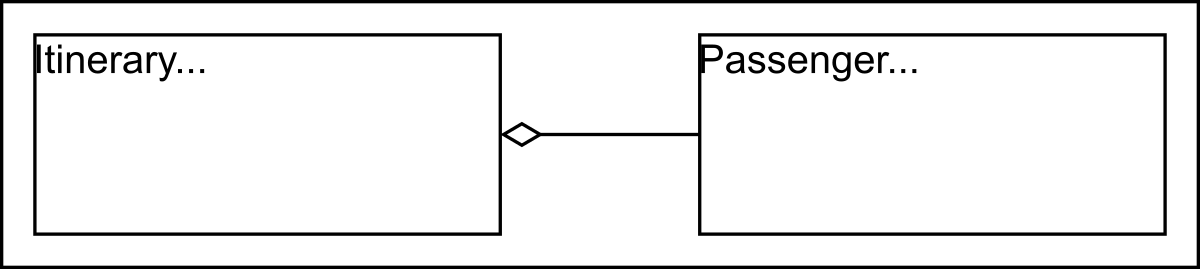
\includegraphics[width=0.5\textwidth]{Images/chapter_25/section_5381527174381568/6639920073670656.png}
 \caption{The aggregation relationship between classes}
\end{figure}

\subsubsection{Composition}\label{HGzFx7hVFvwhfMAlNPkU1}
\\
The class diagram has the following composition relationships:

\begin{itemize}
\item
\protect\phantomsection\label{Xqfs8eZDnECiC8acIZ5h6}
The \texttt{Person} class is composed of the \texttt{Account} class.
\item
\protect\phantomsection\label{52-zH7MqeCivC8X9YV0Gf}
The \texttt{Airline} class is composed of the \texttt{Aircraft} and \texttt{Flight} classes.
\item
\protect\phantomsection\label{atk-W9SRgYjLm4O--Xygt}
The \texttt{Aircraft} class is composed of the \texttt{Seat} class.
\item
\protect\phantomsection\label{pq0DvZVYUQpALomB2H1o5}
The \texttt{Flight} class is composed of the \texttt{FlightInstance} class.
\item
\protect\phantomsection\label{cqMtSh7KTsx-zFgdpdopf}
The \texttt{FlightInstance} class is composed of the \texttt{FlightSeat} class.
\item
\protect\phantomsection\label{fpiiFaCCAjAsQ20ecCxct}
The \texttt{Itinerary} class is composed of the \texttt{FlightReservaion} class.
\end{itemize}

\begin{figure}[htbp]
 \centering
 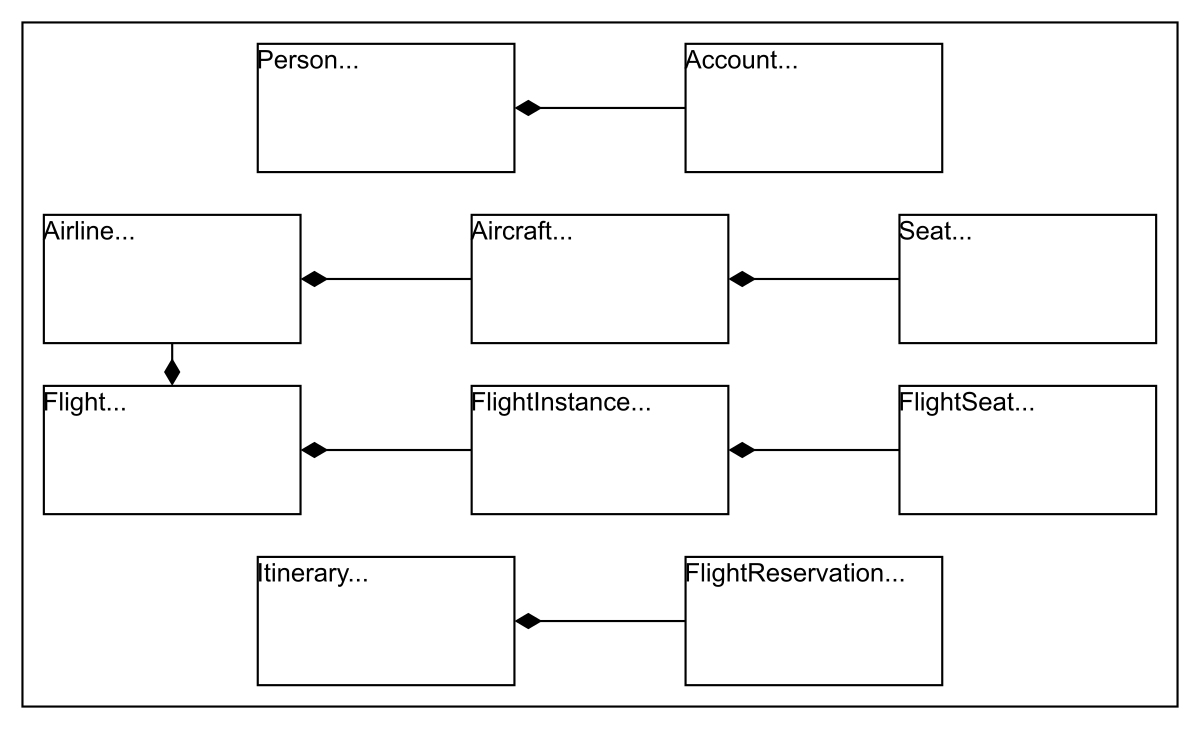
\includegraphics[width=0.5\textwidth]{Images/chapter_25/section_5381527174381568/5092504004067328.png}
 \caption{The composition relationship between classes}
\end{figure}

\subsubsection{Inheritance}\label{J3xemh8Q0u1n_9LNhe1AM}
\\
The following classes show an inheritance relationship:

\begin{itemize}
\item
\protect\phantomsection\label{OfxEEZlsm7h5d_VtamXyM}
The \texttt{Admin}, \texttt{Crew}, \texttt{FrontDeskOfficer}, and \texttt{Customer} classes extend the \texttt{Person} class.
\item
\protect\phantomsection\label{oVBHMd_MgtpQP-LPQpzkh}
The \texttt{FlightSeat} class extends the \texttt{Seat} class.
\item
\protect\phantomsection\label{jPs02km4dxcs3GpculgaW}
The \texttt{CreditCard} and \texttt{Cash} classes extend the \texttt{Payment} class.
\item
\protect\phantomsection\label{-14wn4A0mH1xtIHGk2DcZ}
The \texttt{EmailNotification} and \texttt{SmsNotification} classes extend the \texttt{Notification} class.
\end{itemize}
\begin{quote}
\textbf{Note:} We have already discussed the inheritance relationship between classes in the component section above one by one.
\end{quote}
\subsection{Class diagram of the airline management system}\label{ABmWq73gKOGlcQzOOdsWQ}
\\
In this section, we outline the multiplicity (cardinality) relationships between the main classes in our~airline management system. For each relationship, we explain the allowed number of instances on each side and the real-world or design rationale behind the connection. Understanding these relationships is key to modeling how different entities interact and collaborate to support key workflows in the system.

\begin{longtable}{|p{3cm}|p{3cm}|p{3cm}|p{5cm}|}
\hline
\textbf{Source} & \textbf{Target} & \textbf{Multiplicity} & \textbf{Description} \\
\hline
\endfirsthead
\multicolumn{4}{c}%
{{\bfseries Table continued from previous page}} \\
\hline
\textbf{Source} & \textbf{Target} & \textbf{Multiplicity} & \textbf{Description} \\
\hline
\endhead
\hline \multicolumn{4}{r}{{Continued on next page}} \\
\endfoot
\hline
\endlastfoot

Person & Account & 1 – 1 & Each person has one account \\
Customer & Person & 1 – 1 & Customer inherits from Person \\
Crew & Person & 1 – 1 & Crew inherits from Person \\
FrontDeskOfficer & Person & 1 – 1 & FrontDeskOfficer inherits from Person \\
Passenger & Person & 1 – 1 & Passenger inherits from Person \\
Flight & Airport (departure) & 1 – 1 & Each flight departs from one airport \\
Flight & Airport (arrival) & 1 – 1 & Each flight arrives at one airport \\
Flight & FlightInstance & 1 – 0..* & A flight has multiple instances \\
FlightInstance & FlightSeat & 1 – 0..* & A flight instance has multiple flight seats \\
FlightInstance & Flight & 0..* – 1 & Multiple flight instances relate to one flight \\
FlightInstance & Aircraft & 1 – 1 & Each flight instance uses one aircraft \\
FlightInstance & Crew & 0..* – 0..* & Each flight instance can have multiple crew members \\
Aircraft & FlightSeat & 1 – 0..* & Each aircraft has multiple flight seats \\
Aircraft & FlightInstance & 1 – 0..* & An aircraft is used in multiple flight instances \\
FlightSeat & Seat & 1 – 1 & Flight seat is based on one seat \\
Seat & Aircraft & 0..* – 1 & A seat belongs to one aircraft \\
Airline & Flight & 1 – 0..* & An airline operates multiple flights \\
Airline & Aircraft & 1 – 0..* & An airline owns multiple aircrafts \\
Airline & Crew & 1 – 0..* & An airline has multiple crew members \\
Itinerary & Airport (starting) & 1 – 1 & Itinerary starts at one airport \\
Itinerary & Airport (final) & 1 – 1 & Itinerary ends at one airport \\
Itinerary & FlightReservation & 1 – 0..* & An itinerary includes multiple flight reservations \\
Itinerary & Passenger & 1 – 0..* & An itinerary includes multiple passengers \\
FlightReservation & Passenger & 1 – 0..* & A flight reservation includes multiple passengers \\
FlightReservation & FlightInstance & 1 – 1 & Each reservation is for one flight instance \\
FlightReservation & FlightSeat & 1 – 1 & Each reservation includes one flight seat \\
FlightReservation & Payment & 1 – 1 & Each reservation is paid with one payment \\
Payment & CreditCard & 1 – 0..* & Payments can be made via credit card \\
Payment & Cash & 1 – 0..* & Payments can be made via cash \\
Notification & EmailNotification & 1 – 0..* & Notification via email \\
Notification & SmsNotification & 1 – 0..* & Notification via SMS \\

\end{longtable}

Here's the complete class diagram for our airline management system:

\begin{figure}[htbp]
 \centering
 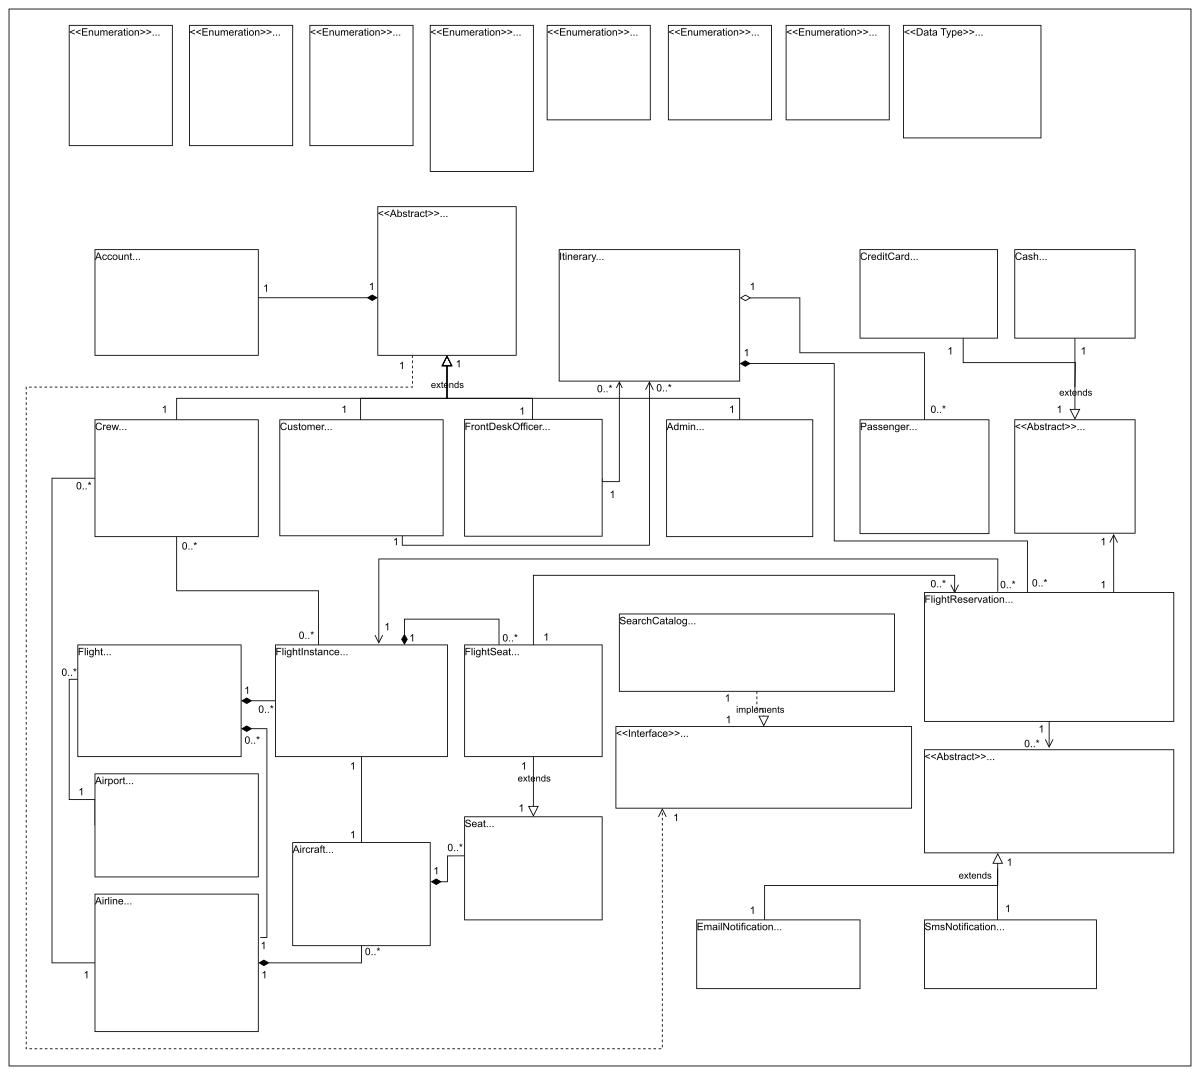
\includegraphics[width=0.5\textwidth]{Images/chapter_25/section_5381527174381568/4768984376147968.png}
 \caption{The class diagram of the airline management system}
\end{figure}

\subsection{Design pattern}\label{H7Qw_4w5E38XhFnWtj4Gj}
\\
To implement the airline management system's core features in a flexible and scalable manner, we apply object-oriented design patterns based on the system\textquotesingle s behavior.

\begin{itemize}
\item
We know that the system sends notifications to users via email or SMS when a reservation is confirmed or a flight is delayed. To model this behavior, we can use the Observer design pattern.
\item
We know that the system allows customers to pay using various methods, such as credit cards or cash. To handle these different payment processes, we can use the Strategy design pattern.
\item
We know that notifications follow a common structure but differ in the way they are delivered (email vs. SMS). To enforce this structure while allowing specific implementations, we can use the Template Method design pattern.
\item
We know that only one instance of the search catalog is needed to manage the flight search system-wide. To ensure this, we can use the Singleton design pattern.
\item
We know that an itinerary may contain multiple flight reservations, and a reservation may include multiple passengers. To treat these collections uniformly, we can use the Composite design pattern.
\item
We know that creating an itinerary involves setting flights, passengers, and payments step by step. To simplify and manage this construction process, we can use the Builder design pattern.
\item
We know that actions like making a reservation, assigning a seat, or processing a payment need to be handled as discrete, trackable tasks. To encapsulate these actions, we can use the Command design pattern.
\item
We are aware that the system generates various types of notifications and payment objects. To manage this object creation logic cleanly, we can use the Factory design pattern.
\end{itemize}

\subsection{AI-powered trainer}\label{JGUc8rBt_30h4xu7w-U3o}
\\
At this stage, everything should be clear. If you encounter any confusion or ambiguity, feel free to utilize the interactive AI-enabled widget below to seek clarification. This tool is designed to help you strengthen your understanding of the concepts.

\begin{figure}[htbp]
 \centering
 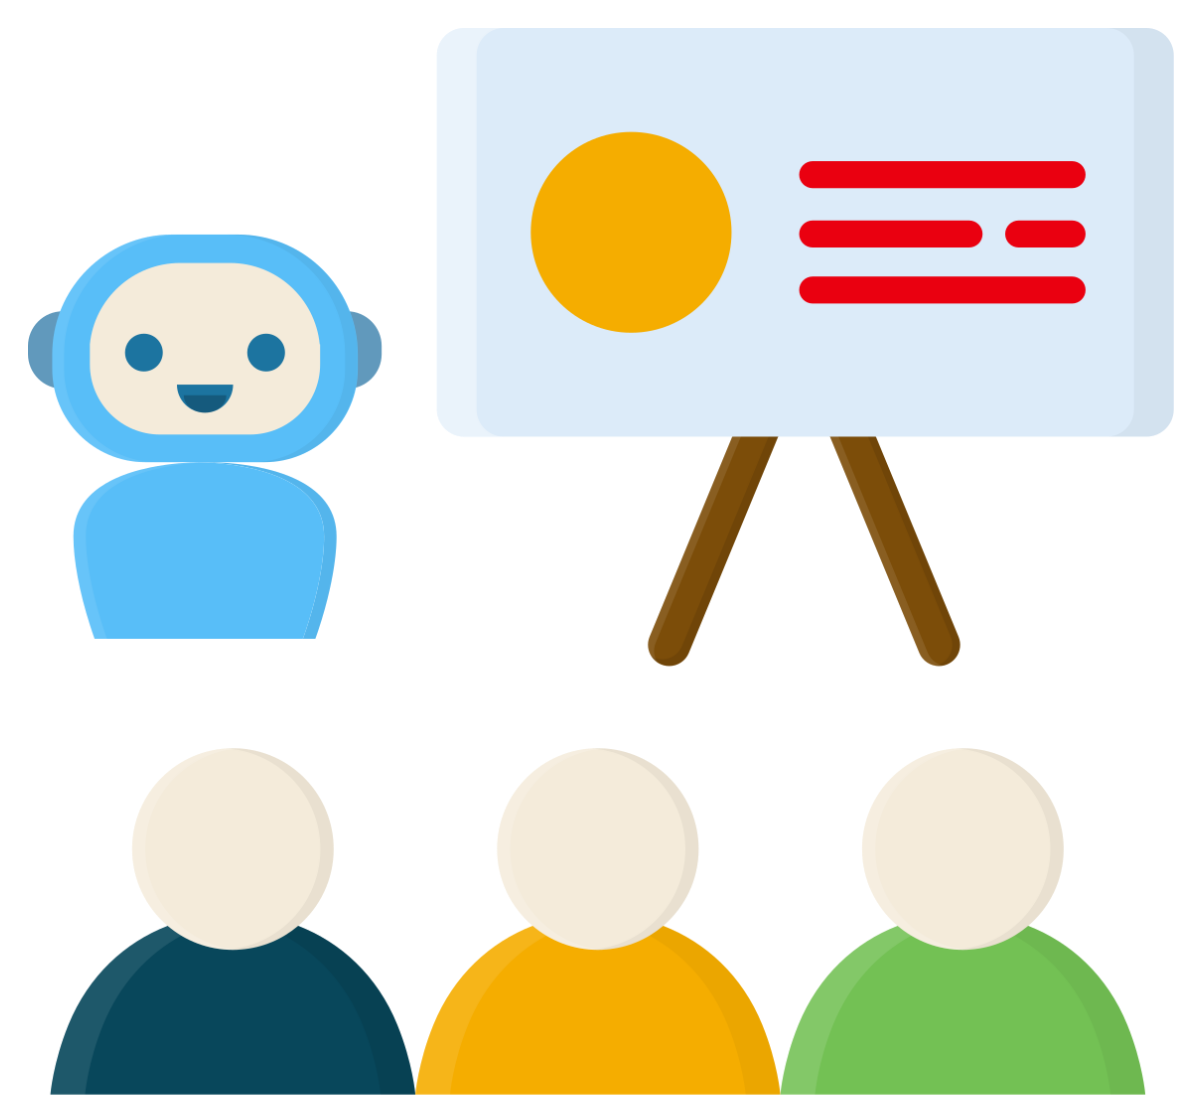
\includegraphics[width=0.15\textwidth]{Images/chapter_25/section_5381527174381568/5489727766396928.png}
 
\end{figure}

We have successfully designed the class diagram for the airline management system. Let 's see how we can construct the sequence diagram for the system in our next lesson.

% End of section content